\documentclass{standalone}
\usepackage{tikzducks}

\begin{document}
	
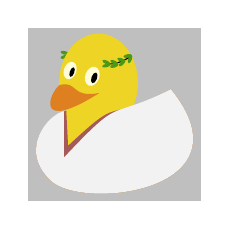
\begin{tikzpicture}
	\fill[gray!50] (0,0) rectangle (2.2,2.2);
		
	\fill[green!50!brown!80!black, rotate around={-15:(0.47,1.88)}] (0.47,1.88) ellipse (0.055 and 0.023);
	\fill[green!50!brown!80!black, rotate around={15:(0.47,1.83)}] (0.47,1.83) ellipse (0.055 and 0.023);
	
	\duck[jacket=red!30!gray]
	
	\begin{pgfinterruptboundingbox}
		\fill[gray!10!white] (0.460,1.140) .. controls (0.267, 1.102) and (-0.125,0.657) .. (0.289,0.261) .. controls (0.704,-0.135) and ( 2.863,0.130) .. (1.818,1.419) .. controls (0.980, 1.000) and ( 1.240,1.378) .. (0.46,0.55) -- cycle;
	\end{pgfinterruptboundingbox}
	
	\draw (1.29,1.82) -- (1.19,1.77) -- (1.1,1.74) -- (1,1.74);

	\fill[green!50!brown!80!black, rotate around={15:(1,1.72)}] (1,1.72) ellipse (0.055 and 0.023);
	\fill[green!50!brown!80!black, rotate around={18:(1.1,1.716)}] (1.1,1.716) ellipse (0.055 and 0.023);
	\fill[green!50!brown!80!black, rotate around={45:(1.2,1.75)}] (1.2,1.75) ellipse (0.055 and 0.023);
	\fill[green!50!brown!80!black, rotate around={70:(1.3,1.8)}] (1.3,1.8) ellipse (0.055 and 0.023);
	
	\fill[green!50!brown!80!black, rotate around={-25:(1,1.76)}] (1,1.76) ellipse (0.055 and 0.023);
	\fill[green!50!brown!80!black, rotate around={-25:(1.1,1.76)}] (1.1,1.76) ellipse (0.055 and 0.023);
	\fill[green!50!brown!80!black, rotate around={-20:(1.19,1.79)}] (1.19,1.79) ellipse (0.055 and 0.023);
	\fill[green!50!brown!80!black, rotate around={10:(1.27,1.84)}] (1.27,1.84) ellipse (0.055 and 0.023);

\end{tikzpicture}	
	
\end{document}